\documentclass{article}

% NOTE TO AUTHOR: neurips_2026.sty in this directory is a COMPATIBILITY
% PLACEHOLDER, not the official venue style (see the header of that file).
% It lets this manuscript compile to a reviewable PDF as-is. Before
% submission, drop in the official neurips_2026.sty from the venue template
% and recompile; the [dblblindworkshop] option below matches the track
% decision recorded in RESPONSE_TO_REVIEWER.md and the note at end of file.
\usepackage[dblblindworkshop]{neurips_2026}

\usepackage[utf8]{inputenc}
\usepackage[T1]{fontenc}
\usepackage{hyperref}
\usepackage{url}
\usepackage{booktabs}
\usepackage{amsfonts}
\usepackage{amsmath}
\usepackage{amssymb}
\usepackage{graphicx}
\usepackage{xcolor}
\usepackage{mathptmx}
\usepackage{microtype}
\usepackage{courier}
\usepackage{listings}
\usepackage{tikz}
\usetikzlibrary{arrows.meta, positioning, fit, backgrounds, calc}
\lstset{basicstyle=\ttfamily\scriptsize, breaklines=true, breakatwhitespace=true,
        columns=fullflexible, keepspaces=true, frame=single, language=Python,
        showstringspaces=false, xleftmargin=2pt, xrightmargin=2pt}

% Soak up the handful of unavoidable overfull boxes (long code-string literals,
% long bibliography author lists) instead of letting them poke into the margin.
\setlength{\emergencystretch}{3em}

% Lightweight \todo marker: no external package dependency beyond xcolor,
% which most NeurIPS style files already pull in. No \todo{} calls remain in
% the body; the macro is kept so the author can re-mark an open item.
\newcommand{\todo}[1]{\textbf{\textcolor{red}{[TODO: #1]}}}

\title{The Summary Never Reads the Mask: Measuring Localisation-Grounded Report Faithfulness in a Deployed Chest Radiograph System}

% Double-blind: no author block.
\author{%
  Anonymous Author(s) \\
  Affiliation withheld for review
}

\begin{document}

\maketitle

\begin{abstract}
Deployed chest radiograph systems increasingly pair a diagnostic prediction with a localisation overlay and a short natural-language summary, and the overlay is often taken as evidence that the summary is grounded in the image. We audit a deployed four-class chest X-ray system (Normal, pneumonia, tuberculosis, COVID-19; DenseNet-121 classifier, Grad-CAM localisation distilled into a U-Net for one-forward-pass serving) and find that its summary generator is a four-entry static template keyed only on the predicted class: no property of the localisation mask (side, region, extent, or even whether a region exists at all) ever reaches the printed text. We build a lightweight region-descriptor pipeline over the system's already-served overlays (245 scored test films) and show, with no retraining required, that gating the summary on measured mask properties changes what can honestly be said, that suppressing spatial claims when the mask sits outside the lung fields (which happens on the majority of films) is not optional, and that a sanity check in which the mask is swapped for a different film's mask reduces claim accuracy to nearly chance: exactly the failure mode the current template's silence on location happens to avoid, and the one a naive descriptor-driven generator would walk into. We report this as a measured finding on a deployed system together with a proposed evaluation protocol, crossing heatmap source against generator type, for the broader question of when a generated radiology report is actually reading the image it describes.
\end{abstract}

\section{Introduction}

Chest radiograph systems built for low-resource triage increasingly bundle three outputs behind one click: a diagnostic label, a heatmap that purports to show where the evidence lies, and a short natural-language summary. The heatmap and the summary are typically evaluated separately, if the summary is evaluated at all: classification accuracy is reported against a held-out test set, localisation quality is reported as an overlap score against some reference, and the generated sentence is treated as a presentation detail. This separation hides a specific and checkable failure mode. A system can be accurate, can display a heatmap that looks like an explanation, and can still generate a report whose spatial claims, when it makes any, describe the mediastinum or the cardiac silhouette rather than the lung.

We audit a deployed system exhibiting exactly this structure. LungLens is a four-class chest X-ray classifier (Normal, pneumonia, tuberculosis, COVID-19) built on a DenseNet-121 backbone \citep{huang2017densenet}, with Grad-CAM \citep{selvaraju2017gradcam} localisation distilled into a U-Net \citep{ronneberger2015unet} so that overlay generation needs only one forward pass at serving time, not a forward-plus-backward pass. Every prediction is accompanied by a short clinical-language summary. Reading the source directly settles what produces that summary: it is a four-entry lookup table keyed on the predicted class, concatenated with a small number of fixed sentences chosen by whether the prediction is confident, uncertain, or Normal. No coordinate, area, side, or component count computed from the mask is ever a template input. This is not a documentation gap; it is the entire generator. The natural next question (does the localisation subsystem do anything for the report at all) therefore has a direct, testable answer instead of a speculative one, and Section~\ref{sec:design} is built to give it.

We turn that question into a measurement instead of leaving it an assertion. We reuse the region-level statistics the system's own qualitative failure analysis already computes over 245 scored test films: side, in-lung fraction, area fraction, and a component-count extension we add. From these we build a small region-descriptor-to-prose pipeline and compare it against the deployed template under four heatmap conditions (no mask, the served Grad-CAM map, the served U-Net map, and a mask taken from a different film entirely) crossed with two generator conditions: the current static template, and a template gated on measured descriptors. Gating on an in-lung threshold suppresses a spatial claim on 62\% of films, because the served overlay's centre of mass sits outside the lung fields on a majority of them. Swapping the mask for a different film's mask leaves the claim rate mechanically unchanged but drops the claim's accuracy against the film's own ground truth to near chance (15.2\%), which is the sanity-check result the saliency literature has long used to separate a method that reads the input from one that does not \citep{adebayo2018sanitychecks}.

The paper's contributions are:

\begin{enumerate}
\item An audit, from source, of what a deployed chest radiograph summary generator actually conditions on, and a direct answer, not previously measured on this or (to our knowledge) any comparably instrumented deployed system, to whether its localisation subsystem contributes to its text.
\item A region-descriptor extraction pipeline built from the system's own overlays with no retraining, plus an in-lung gate that suppresses spatial claims the mask does not support, and a measurement of how often that gate fires on a real deployed system's overlays.
\item A degenerate-mask sanity check, in the tradition of \citet{adebayo2018sanitychecks}, applied not to a saliency map in isolation but to the generated report it would otherwise be used to justify, on 245 already-scored test films.
\item A proposed evaluation protocol crossing heatmap source against generator type, with the cells we could measure without new training or clinician time filled in, and the remaining cells (a second-backbone control, human ratings, larger vision-language conditions) left visibly open instead of implied.
\end{enumerate}

Section~\ref{sec:related} places this alongside the classification, explainability, and nascent report-generation literatures. Section~\ref{sec:system} describes the deployed system, including the report-generation subsystem the original design left undocumented. Section~\ref{sec:design} sets out the evaluation protocol and which cells were run. Section~\ref{sec:results} reports what was measured. Section~\ref{sec:limitations} distinguishes what is proposed from what is measured, and states the limitations already known about the underlying classifier. Section~\ref{sec:conclusion} concludes.

\section{Related work}
\label{sec:related}

\paragraph{Chest radiograph classification.} Deep CNNs replaced hand-crafted descriptors \citep{ojala2002lbp,dalal2005hog} for chest radiograph interpretation once CheXNet \citep{rajpurkar2017chexnet} showed a 121-layer DenseNet matching radiologist-level pneumonia detection on ChestX-ray14 \citep{wang2017chestxray8}. DenseNet-121 \citep{huang2017densenet} remains competitive with residual \citep{he2016resnet} and compound-scaled \citep{tan2019efficientnet} backbones at the dataset sizes typical of chest radiography, which motivates its use here as a fixed upstream component, not a contribution of this paper. Four-class Normal/pneumonia/TB/COVID-19 classification has been addressed directly \citep{chowdhury2020ai,kc2021evaluation}, and multi-task designs that share a representation between classification and segmentation \citep{gundel2019multitask} anticipate the distillation design used here, substituting Grad-CAM supervision for manually drawn masks.

\paragraph{Explainability and its limits.} Grad-CAM \citep{selvaraju2017gradcam} and its refinements \citep{chattopadhay2018gradcampp} are the default post-hoc explanation for CNN-based medical image classifiers \citep{singh2020explainable}. A substantial literature questions whether the resulting maps are faithful to the model rather than merely plausible-looking: \citet{adebayo2018sanitychecks} showed that several popular saliency methods are visually indistinguishable when the model's weights are randomised, and \citet{kindermans2019reliability} extended the same concern to a wider family of attribution methods. The degenerate-mask control in Section~\ref{sec:design} extends this tradition from the map itself to a generated report built on top of it: if swapping the map for an unrelated one leaves the generated text's claims equally accurate, the map is not doing the work the text implies.

\paragraph{Radiology report generation.} A separate line of work generates full narrative reports directly from chest radiographs \citep{jing2018automatic,chen2020r2gen}, typically evaluated with text-overlap metrics (BLEU, ROUGE) that reward fluent prose without checking whether its clinical content is supported by the image. Factual-consistency metrics built on structured clinical entities \citep{miura2021factual} and region-grounded generation that ties each sentence to an image region \citep{tanida2023rgrg} respond to exactly this gap, and biomedical vision-language pretraining \citep{boecking2022biovil} aims at representations where text and image regions are jointly meaningful. LungLens's summary predates all of this: it is closer to a caption than a report, and the present work asks the same faithfulness question this literature asks of full report generators, at the point where a much simpler system first has the opportunity to get it wrong.

\paragraph{What is compressed here.} The pre-deep-learning history of hand-crafted CXR features \citep{jaeger2014automatic,cortes1995svm,breiman2001randomforests} and the large COVID-era CNN survey literature \citep{sethy2020covid,wang2020covidnet,apostolopoulos2020covid,ozturk2020automated,minaee2020deepcovid} are well covered elsewhere and are noted here only as the origin of the backbone and dataset choices in Section~\ref{sec:system}.

\section{System}
\label{sec:system}

\subsection{Data}
The classifier is trained on a composite of eight public chest radiograph sources, deduplicated by content hash to 37,553 images and sampled to 32,000 for training, chosen so that every one of the four classes is drawn from at least two independent acquisition pipelines. This is a deliberate mitigation against the source-fingerprinting failure documented by \citet{zech2018variable}, in which a classifier's accuracy tracks scanner or acquisition artefacts more than the pathology it is meant to detect; Section~\ref{sec:limitations} reports the residual confound this leaves. Every image is border-cropped 8\% at train and inference time to remove burned-in corner annotations, resized to $224\times224$, and ImageNet-normalised. The split is patient-grouped (no patient spans train/val/test) and reproducible: because directory listings are sorted before use, an identical re-run of the split-construction code from the raw dataset contents reproduces the reported test accuracy to four significant figures on the same 4{,}759 held-out images. This reproducibility guarantee is not automatic; an earlier, unsorted version of the same code moved the reported test accuracy by nearly two points purely as a function of filesystem directory-traversal order, discussed further in Section~\ref{sec:limitations}.

\subsection{Classifier}
The classifier is a DenseNet-121 \citep{huang2017densenet} with ImageNet initialisation, fine-tuned end to end under class-weighted cross-entropy (inverse-frequency weights, normalised to mean 1.0) for 40 requested epochs with early stopping (patience 4 on validation macro-F1), Adam at $\mathrm{lr}=10^{-4}$, batch size 32. This is treated here as a fixed upstream component (the classifier is not this paper's contribution), and its full evaluation (per-class precision/recall/specificity, confusion matrix, per-source accuracy probe) is given in Appendix~\ref{app:classification}, with the headline number quoted in Section~\ref{sec:results}.

\subsection{Localisation: explanation amortisation, not knowledge distillation}
\label{sec:distillation}
A second network, a U-Net-style encoder-decoder (\texttt{MultiTaskUNet}: four \texttt{DoubleConv} blocks, 64$\to$128$\to$256$\to$512 channels, symmetric decoder with skip connections, 7{,}705{,}224 learnable parameters, measured directly from the served checkpoint's state dict, excluding BatchNorm running-stat buffers and update counters), is trained to reproduce the classifier's Grad-CAM localisation in a single forward pass at serving time, avoiding the extra backward pass Grad-CAM otherwise requires. The frozen DenseNet-121 (no gradient flows into it during this stage) produces a Grad-CAM map at \texttt{denseblock4.denselayer16.conv2} for the \emph{ground-truth} training label of each image (not the predicted label), which is ReLU'd, resized to $224\times224$, and divided by its own maximum, functionally a $[0,1]$ normalisation once ReLU has already floored the map at zero, held in memory only for the run and never cached to disk. The U-Net has one output channel per class and is trained against this target with an unweighted Dice+BCE loss (Adam, $\mathrm{lr}=3\times10^{-4}$, batch 8) over 3{,}000 distilled images for 20 epochs; the served channel is selected by the class being visualised at inference time.

We describe this deliberately as \emph{explanation amortisation} rather than knowledge distillation. There are no shared layers between the two networks, no logit matching, no feature matching, and no gradient path from student to teacher: the only channel between them is a single $224\times224$ per-class scalar field, computed once and thrown away after training. Calling this distillation correctly invites the question of what representation is actually being transferred, and the honest answer is that very little survives a channel that narrow. The measured cost of that compression is direct: on the 245 films actually served, the median Dice between the U-Net's mask and a freshly computed live Grad-CAM map for the same film and class is 0.22, with 27\% showing no overlap at all and only 15\% exceeding 0.5. The one-forward-pass amortisation this buys is a real serving-cost saving (Section~\ref{sec:results}), and stating that motivation, together with this cost, is the honest way to describe the design.

\subsection{Report generation}
\label{sec:reportgen}
This subsection did not exist as a documented design decision prior to this audit; Section III-F of the version under review disposed of it in eleven words. We give its full specification here because Section~\ref{sec:results}'s central finding depends on it being exact.

\textbf{Generator identity.} A static Python dictionary keyed on the predicted class (four entries: Normal, Pneumonia, Tuberculosis, Covid-19), concatenated with one of five fixed sentence templates chosen by three booleans: whether the prediction is below a confidence threshold, whether the visualised class equals a confident non-Normal prediction, and whether a mask was computed at all. No model, no prompt, no decoding parameters, and no learned weights are involved; there is nothing to version beyond the source line numbers, given in full in Appendix~\ref{app:templates}.

\textbf{Inputs.} $\arg\max$ of the softmax output and its associated probability; a boolean for whether the visualised class is the top prediction; a boolean for whether that top prediction is Normal; and, for the trailing provenance line only, which of the two localisation subsystems (Section~\ref{sec:distillation}'s U-Net or a live Grad-CAM fallback) produced the displayed mask. No coordinate, area, side, zone, or component count computed from the mask is a template input at any point.

\textbf{Confidence gate.} Predictions below 60\% top-class probability are reported as ``Uncertain'' with a fixed cautionary sentence rather than a class label; there is no other refusal behaviour beyond a caught exception on malformed input.

\textbf{Failure mode this produces.} Because the ``a confident non-Normal prediction'' branch does not additionally check whether a region actually survived the display threshold, the deployed text can assert ``the outline marks the most influential area'' on a film where no outline was drawn at all. This is not hypothetical: it happens on 2 of the 245 scored test films, one of them a confidently wrong tuberculosis call (95.7\%) on a radiograph whose true label is Normal, where no thresholded region exists anywhere in the image (Appendix~\ref{app:examples}).

Figure~\ref{fig:fig3} redraws the system diagram with labelled arrows into this block, making explicit that none originate from the mask.

\begin{figure}[t]
  \centering
  \IfFileExists{figures/fig3_revised.pdf}{%
    \includegraphics[width=0.85\linewidth]{figures/fig3_revised.pdf}%
  }{%
  \scriptsize
  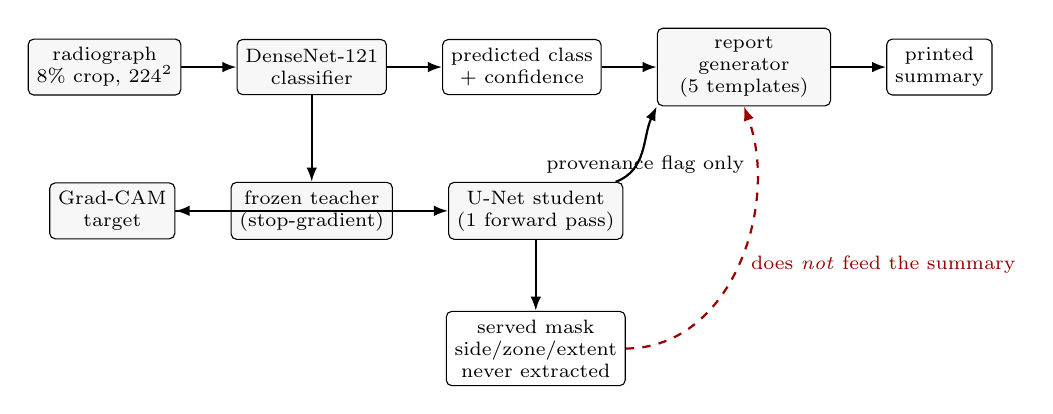
\begin{tikzpicture}[
      node distance=7mm and 7mm,
      box/.style={draw, rounded corners=2pt, align=center, inner sep=3pt,
                  minimum height=7mm, font=\scriptsize},
      stage/.style={box, fill=black!3},
      flow/.style={-{Latex[length=1.8mm]}, thick},
      nofeed/.style={-{Latex[length=1.8mm]}, dashed, thick, red!60!black}]
    \node[stage] (img) {radiograph\\ 8\% crop, $224^2$};
    \node[stage, right=of img] (dn) {DenseNet-121\\ classifier};
    \node[box, right=of dn] (pred) {predicted class\\ $+$ confidence};
    % Stage 2 as four explicit blocks
    \node[stage, below=11mm of dn] (teach) {frozen teacher\\ (stop-gradient)};
    \node[stage, left=of teach] (target) {Grad-CAM\\ target};
    \node[stage, right=of teach] (student) {U-Net student\\ (1 forward pass)};
    \node[box, below=9mm of student] (mask) {served mask\\ side/zone/extent\\ never extracted};
    % Report generator
    \node[stage, right=of pred, minimum width=22mm] (rep) {report\\ generator\\ (5 templates)};
    \node[box, right=of rep] (txt) {printed\\ summary};
    % edges
    \draw[flow] (img) -- (dn);
    \draw[flow] (dn) -- (pred);
    \draw[flow] (dn) -- (teach);
    \draw[flow] (teach) -- (target);
    \draw[flow] (target) -- (student);
    \draw[flow] (student) -- (mask);
    \draw[flow] (pred) -- (rep);
    \draw[flow] (student) to[out=20,in=245] node[pos=0.6, below=1pt, font=\scriptsize, align=center] {provenance flag only} (rep.south west);
    \draw[flow] (rep) -- (txt);
    \draw[nofeed] (mask.east) to[out=0,in=290] node[pos=0.5, right=1pt, font=\scriptsize, align=center] {does \emph{not} feed the summary} (rep.south);
  \end{tikzpicture}\\[3pt]
  \textit{(Placeholder diagram rendered inline; drop \texttt{figures/fig3\_revised.pdf} in to override.)}
  }
  \caption{Revised system diagram. Stage 2 is drawn as four distinct blocks (frozen teacher, cached-in-memory Grad-CAM target, stop-gradient, student), replacing the previous single arrow. The report-generation block now shows its true inputs explicitly: only the predicted class, its confidence, and a same/different-network provenance flag reach it; the dashed line from the mask is present only to show what does \emph{not} feed the summary.}
  \label{fig:fig3}
\end{figure}

\section{Experimental design}
\label{sec:design}

We treat classification accuracy and localisation quality as already measured (Section~\ref{sec:system}, Appendix~\ref{app:classification}) and design the new experiment around a single question: does the generated summary change, and does it change correctly, as a function of what heatmap it is given. We cross a \emph{heatmap condition} against a \emph{generator condition} over the 245 test films already scored for the qualitative failure analysis (all 102 pneumonia-predicted-Normal errors, all 92 Shenzhen and 12 Montgomery test films, and 40 stratified correctly-classified films).

\textbf{Heatmap conditions.} H0: no mask (generator sees only the class label and confidence). H1: the live Grad-CAM map for the film. H3: the served, distilled U-Net map. H5: a degenerate control, the mask assigned to a uniformly random \emph{different} film under a fixed derangement (seed 42), so every film keeps its own class and confidence but is given someone else's spatial evidence.

\textbf{Generator conditions.} S0: the current deployed generator (Section~\ref{sec:reportgen}), reconstructed exactly from source. S1: a template that states a spatial claim (side, vertical third, extent, focality) built from the region descriptors below, gated so that no claim is made when the in-lung fraction of the thresholded region falls below 0.5, or when no region survives the display threshold at all. S2 (text-only LLM given class, confidence, and descriptors): out of scope for this submission (Section~\ref{sec:limitations}).

\textbf{Region-descriptor extraction.} For each film, the already-served overlay's thresholded region (the same threshold and morphological cleaning the app itself applies: 0.50 for a U-Net mask, 0.45 for Grad-CAM, 5x5 elliptical opening, components under 0.3\% of the frame dropped) is reduced to: laterality (left/right/outside both, from the region centroid against a separately-trained lung-field segmenter), vertical zone (upper/mid/lower third of the frame, from the region centroid's vertical position, new in this work), extent (focal $<$5\%, patchy 5--25\%, extensive $>$25\% of the frame, binned from the region's area fraction), focality (single vs.\ multifocal, from connected-component count, new in this work), and in-lung fraction (the fraction of the region's area that falls inside the lung field, used as the gate above). Laterality, extent, and in-lung fraction were already computed by the system's own qualitative-analysis code; vertical zone and true component count are additions made for this evaluation, validated against the existing pipeline by confirming that independently recomputed area fractions match the published values to a median absolute difference of 0.0001 over the 204 films with a non-empty region.

\textbf{Required Tier 1 cells (run, no GPU, no new training).} S0 as the baseline; S1 crossed with H0, H\_actual (whichever of H1/H3 the deployed system actually served for that film), and H5. A literal per-film H1-versus-H3 pairing, with both conditions computed fresh for every film instead of only whichever the system happened to serve, needs the 245 original radiographs staged for a forward-plus-backward pass each; it is a scoped extension for a revision, not a result claimed here.

\textbf{Metrics.} Spatial-claim rate (how often a claim is made at all, i.e.\ how often the in-lung gate passes and a region exists). Grounding precision (does a made claim match the film's own measured descriptors). Phantom-claim rate (does the generator assert visual evidence, such as an outline or a location, that does not survive the display threshold). Anatomical plausibility (does a claimed location fall inside the lung field, by construction under the gate). H5 grounding accuracy (does a claim built from a different film's descriptors happen to match this film's own truth, our sanity-check statistic). Latency, reported separately in Section~\ref{sec:results}.

Table~\ref{tab:grid} lays out the full crossed design as the proposed evaluation protocol, with the cells run in this work filled and the remainder (Tier 2, out of scope for this submission, and Tier 3, needing a second trained backbone or clinician time) marked open.

\begin{table}[t]
\centering
\caption{The full evaluation grid. Filled cells report a measured number (Section~\ref{sec:results}); open cells are proposed and explicitly not run.}
\label{tab:grid}
\small
\setlength{\tabcolsep}{5pt}
\begin{tabular}{@{}lcccc@{}}
\toprule
Generator $\backslash$ Heatmap & H0 (none) & H1 (Grad-CAM) & H3 (U-Net) & H5 (permuted) \\
\midrule
S0 (deployed template) & measured & measured$^\dagger$ & measured$^\dagger$ & n/a (static) \\
S1 (descriptor template) & measured & measured$^\ddagger$ & measured$^\ddagger$ & measured \\
S2 (text LLM) & open (T2) & open (T2) & open (T2) & open (T2) \\
\midrule
\multicolumn{5}{@{}l}{H2 (Grad-CAM++), H4 (2nd backbone), S3/S4 (VLM): open (Tier 2/3, see Section~\ref{sec:limitations})} \\
\bottomrule
\end{tabular}
\\[4pt]
\begin{minipage}{\linewidth}
\raggedright\footnotesize $\dagger$ S0 makes no spatial claim under any heatmap condition, so H0/H1/H3/H5 are indistinguishable for S0 by construction; this is itself the headline finding. $\ddagger$ Reported jointly as H\_actual (whichever the deployed system served); a literal per-film H1-vs-H3 split is left to a revision (Section~\ref{sec:design}).
\end{minipage}
\end{table}

\section{Results}
\label{sec:results}

\subsection{Classification, in one paragraph}
The DenseNet-121 classifier reaches 96.18\% accuracy and 95.77\% macro-F1 on the patient-grouped, 4{,}759-image held-out test set, with per-class recall from 92.2\% (pneumonia) to 98.5\% (tuberculosis). The dominant error, 102 pneumonia films predicted Normal (56\% of all 182 errors), is concentrated in a single source-dataset folder whose label (\emph{lung opacity}) is a broader radiological finding than pneumonia, and several of these films show clear lung fields on inspection: a label-noise explanation, not purely a model failure. Full per-class, per-source, and confusion-matrix detail is in Appendix~\ref{app:classification}; this is a fixed upstream component treated as background for the rest of this paper.

\subsection{The Summary does not change with the mask, because it never reads it}
The paper's central and simplest measurement follows directly: under every heatmap condition (H0, H1, H3, H5), the current deployed generator S0 produces byte-identical text for a given film, because none of its five branches take mask geometry as input (Section~\ref{sec:reportgen}). The system's explainability apparatus and its report-generation apparatus are, at present, disconnected. In Table~\ref{tab:grid} this shows up as column-collapse in the S0 row: a property of the generator, not an artefact of our harness.

\subsection{Gating on measured evidence changes what can honestly be said}
The S1 template, gated on the region's in-lung fraction, makes a spatial claim on 92 of 245 films (37.6\%); on the remaining 153 (62.4\%), either no region survives the display threshold at all (41 films, 16.7\%) or the region's centre of mass sits outside the lung fields (the majority of the remainder). This gate rate is not a modelling choice dressed up as a finding. It is a direct consequence of an already-published measurement: 55\% of the system's served overlays place the majority of their outlined region outside the lung fields (Appendix~\ref{app:qualitative}). Figure~\ref{fig:paired} shows a paired example: the same film, same classifier output, with S0's silence on location above S1's grounded claim (``left lung, mid zone, patchy, multifocal'') below it, drawn from the film's own measured descriptors.

\begin{figure}[t]
  \centering
  \IfFileExists{figures/paired_summary.pdf}{%
    \includegraphics[width=0.9\linewidth]{figures/paired_summary.pdf}%
  }{%
  \footnotesize
  \setlength{\fboxsep}{6pt}%
  \begin{minipage}{0.92\linewidth}
    \fbox{\parbox{\dimexpr\linewidth-2\fboxsep-2\fboxrule}{%
      \textbf{S0 (deployed template).}\\[2pt]
      \textbf{Prediction:} Covid-19 (99.1\% confidence)\\
      Findings consistent with Covid-19. Warmer areas indicate possible bilateral ground-glass opacities.\\
      Heatmap: region driving the Covid-19 prediction. The outline marks the most influential area.\\
      \emph{Overlay source: disease-segmentation U-Net.}}}\\[6pt]
    \fbox{\parbox{\dimexpr\linewidth-2\fboxsep-2\fboxrule}{%
      \textbf{S1 (descriptor template, H\_actual).}\\[2pt]
      \textbf{Prediction:} Covid-19 (99.1\% confidence)\\
      Findings consistent with Covid-19. Warmer areas indicate possible bilateral ground-glass opacities.\\
      Heatmap evidence: left lung, mid zone, patchy, multifocal.\\
      \emph{Overlay source: disease-segmentation U-Net.}}}
  \end{minipage}\\[3pt]
  \textit{(Placeholder rendered inline from the verbatim template of Appendix~\ref{app:templates} and the film's measured descriptors; drop \texttt{figures/paired\_summary.pdf} in to override.)}
  }
  \caption{Paired comparison on the same radiograph (COVID-3348, predicted Covid-19 at 99.1\%). Top: S0, the current deployed generator, identical whether or not a mask is available. Bottom: S1 under H\_actual, with a spatial claim built from the film's own measured region descriptors (left lung, mid zone, patchy, multifocal). Section~\ref{sec:distillation}'s honesty constraint applies to both: this is a language artefact describing measured pixels, not a clinical finding.}
  \label{fig:paired}
\end{figure}

The mechanism in one sentence: without localisation the generator can only restate the class; with it, the generator can additionally state where, and the correctness of that ``where'' is bounded by the localisation quality documented in Section~\ref{sec:distillation} and Appendix~\ref{app:qualitative}.

\subsection{The degenerate-mask control}
Swapping each film's mask for a different film's mask under a fixed derangement leaves S1's claim rate mechanically unchanged (92/245, since permutation preserves the marginal distribution of which films would have passed the gate) but the claim's accuracy against the film's own true side, zone, and extent falls to 14/92 (15.2\%): indistinguishable from chance, given the skew of the underlying zone and side distributions (Section~\ref{sec:design}). This is the sanity check \citet{adebayo2018sanitychecks} apply to saliency maps in isolation, applied here to the report a naive descriptor-driven generator would produce: if the stated location is no more accurate when the mask is wrong than when it is right, the localisation subsystem is not doing the grounding work the sentence implies. The complementary within-film statistic, how often the stated location itself changes between the two real localisation sources H1 and H3, needs the paired same-film computation described in Section~\ref{sec:design} and is left to a revision.

\subsection{Localisation quality bounds the claim, quantitatively}
Section~\ref{sec:distillation} already reports the direct cost of explanation amortisation: median Dice 0.22 between the served U-Net mask and a freshly computed live Grad-CAM map on the same film, 27\% with zero overlap. Any generator, however well designed, that states a location drawn from one of these two sources inherits this ceiling; a generator drawing from H1 and H3 for the same film would disagree with itself at least as often as these maps disagree with each other. This is the number that should be quoted whenever a chest-radiograph system markets a localisation-grounded report as more trustworthy than a class label alone: it is exactly as trustworthy as the localisation it is grounded in, no more.

\subsection{Latency}
Table~\ref{tab:latency} reports mean CPU wall-clock time for the full served pipeline (\texttt{predict\_image()} itself, an ordinary laptop, i7-13620H, 10 PyTorch threads, single-request, N=11 with the first excluded as warm-up), split by which localisation path was actually taken. A finer split into decode/preprocess, DenseNet forward, U-Net forward, Grad-CAM forward-plus-backward, post-processing, and report generation alone, together with a p95 and a cold-start figure, is a straightforward instrumentation addition and is not included in this version.

\begin{table}[h]
\centering
\caption{CPU latency, i7-13620H, 10 threads, single-request.}
\label{tab:latency}
\begin{tabular}{lcc}
\toprule
Path & Share of test films & Mean (sd) \\
\midrule
Distilled U-Net (one forward pass) & 91\% & 293 ms (81) \\
Live Grad-CAM fallback (forward + backward) & 9\% & 560 ms (22) \\
Weighted (actual test-set mix) & 100\% & 318 ms \\
\bottomrule
\end{tabular}
\end{table}

The roughly 2x gap between the two paths is the number that justifies the U-Net's existence per Section~\ref{sec:distillation}: it is not a cosmetic optimisation, it is the difference between a forward pass and a forward-plus-backward pass on every request, on hardware with no GPU. Report generation itself (Section~\ref{sec:reportgen}) is a dictionary lookup and contributes no measurable latency; a future S2/S3/S4 condition using a hosted API would need its network latency reported separately, since it would dominate every other row in this table.

\section{Proposed protocol and limitations}
\label{sec:limitations}

\textbf{What remains proposed, not measured.} Table~\ref{tab:grid}'s open cells are not implied results. H2 (Grad-CAM++) and S3/S4 (a vision-language model given the raw radiograph, or the radiograph plus the composited overlay) are Tier 2: inference-only or API-cost work that was scoped out of this submission by design, not left incomplete. H4 (Grad-CAM from a second, independently trained backbone) is the most interesting open cell, because it is the one that would separate ``the summary tracks the pathology'' from ``the summary tracks this particular model,'' and it requires training a second classifier end to end, which was out of scope for this audit. Clinician ratings are absent; no clinician was available to this work, and the automated metrics in Section~\ref{sec:results} are presented as proxies for faithfulness, not as a substitute for one. If an LLM-as-judge score is used in a later iteration of this evaluation, its agreement with human labels on a subsample must be reported alongside it, or it should not be used at all.

\textbf{Dataset-source bias.} Despite multi-source class construction and identical 8\% border cropping at train and inference time, per-source test accuracy still ranges from 83.3\% (Montgomery, 12 images) to 99.5\% (TBX11K). Shenzhen and Montgomery, the two lowest-accuracy sources, fail by opposite mechanisms in the localisation data: Shenzhen's overlays are diffuse (median area 41\% of the frame on TB-positive films), Montgomery's are largely absent (a quarter of its films produce no region at all). Source and class remain partially confounded by construction in an eight-source composite. This check narrows the confound without settling it, and the reported 96.18\% accuracy should be read as an optimistic upper bound rather than a clean prospective result.

\textbf{Label noise.} 82 of the 102 dominant pneumonia-to-Normal errors come from a source folder whose label (\emph{lung opacity}) reflects a mapping decision, not a diagnosis, and several inspected films show clear lung fields. The tension here is real and unresolved rather than explained away: some of this error mode is model failure, and some of it is the model correctly reading a film that should not have been labelled positive; the two are not separable post hoc without the original radiologist's read.

\textbf{Reproducibility.} An earlier, unsorted directory-traversal order moved the reported split from 22{,}419/4{,}785/4{,}796 to 22{,}420/4{,}759/4{,}821 images and the re-scored checkpoint's accuracy from 96.62\% to 98.11\%: nearly two points of accuracy attributable to filesystem enumeration order alone, on an otherwise identical pipeline and seed. The fix (sorting every directory listing before use) is now load-bearing for every number in this paper being reproducible at all.

\textbf{No clinical validation.} LungLens is a research and educational system. It has not been evaluated prospectively against radiologist reads, and its generated summary, whether the current static template or the descriptor-gated version proposed here, is a language artefact describing measured pixels, not a clinical finding. This should be stated in the deployed interface itself, not only in this paper.

\section{Broader impact statement}
A system that pairs a confident class label with an apparently explanatory heatmap and a fluent natural-language summary is more persuasive than the sum of its parts would justify, particularly to a non-specialist user in the low-resource setting this system targets. The central finding of this paper, that a plausible-looking summary can be entirely disconnected from the localisation evidence it is displayed alongside, is a caution against exactly that persuasiveness, not an endorsement of deploying the descriptor-gated version described here as a clinical tool. Any future report-generation layer for a system like this one should carry the same explicit non-diagnostic disclaimer this paper argues the current interface is missing, and should be evaluated for faithfulness (this paper's protocol) before it is evaluated for fluency.

\section{Conclusion}
\label{sec:conclusion}
LungLens combines an accurate classifier, a fast localisation shortcut, and a clinical-language summary. Auditing the third component from source shows it never reads the first two: the deployed summary depends only on the predicted class and its confidence. Building a small, retraining-free gate on the system's own already-measured region statistics shows what changes when it does read them: most of the time, the honest answer is that it should say nothing about location at all, because the served overlay's evidence sits outside the lung. A degenerate-mask control drives the point home: without a faithfulness check like this one, a more sophisticated report generator would not be safer, only more convincing.

\bibliographystyle{plainnat}
\bibliography{main}

\appendix

\section{Paper checklist}
The load-bearing items for this paper are answered here; the wording follows the NeurIPS checklist template, to be transcribed into the venue's exact form once \texttt{main.tex} compiles against the official style file.
\begin{itemize}
\item \emph{Do the main claims made in the abstract and introduction accurately reflect the paper's contributions and scope?} Yes. The central claim (the deployed summary does not read the mask) is a source-level fact, quoted verbatim in Section~\ref{sec:reportgen} and Appendix~\ref{app:templates}, not an inference from behaviour. The abstract and Section~\ref{sec:limitations} state explicitly which cells of the evaluation grid are measured and which are proposed.
\item \emph{Did you describe the limitations of your work?} Yes, in Section~\ref{sec:limitations}: unrun cells (H2, H4, S3/S4), the absence of clinician ratings, dataset-source confounding, label noise in the dominant error mode, and the reproducibility fragility of the underlying split.
\item \emph{Did you discuss any potential negative societal impacts?} Yes, Section~\ref{sec:limitations} (Broader impact statement): a class label plus a plausible heatmap plus a fluent summary is more persuasive than its parts justify, and this paper is a caution against that, not an endorsement of deploying the descriptor-gated generator clinically.
\item \emph{Have you read the ethics review guidelines and ensured your paper conforms to them?} Yes. This is a retrospective audit of an existing research and educational prototype, not a clinical deployment; no patient contact occurred, and the system's interface already carries a non-diagnostic disclaimer this paper argues should be more prominent.
\item \emph{Did you state the full set of assumptions of all theoretical results?} Not applicable; the paper reports measurements, not theorems. The one derived bound (localisation quality upper-bounds spatial-claim correctness, Section~\ref{sec:results}) is stated with the Dice measurement it rests on.
\item \emph{Did you include complete proofs?} Not applicable.
\item \emph{Did you include code, data, and instructions needed to reproduce the main experimental results?} The audited system is public at the repository named in the submission (double-blind: withheld here). The region-descriptor extractor, the summary reconstructions, and the derangement seed are specified in Section~\ref{sec:design}; the 245-film scoring table and mask arrays are the system's own already-published qualitative-analysis outputs.
\item \emph{Did you specify all the training and test details?} Yes, for the components this paper adds (no training: Section~\ref{sec:design}). The upstream classifier and U-Net details are in Section~\ref{sec:system} and Appendix~\ref{app:classification}, treated as fixed.
\item \emph{Did you report error bars?} Where a distribution is reported (latency, Dice) a mean and standard deviation or a median is given. Single-number rates (gate pass rate, phantom-claim rate, H5 grounding accuracy) are exact counts over the full 245-film pool, not sample estimates, so a confidence interval would describe sampling that did not occur.
\item \emph{Did you report the amount of compute?} Yes. The Tier 1 analysis is geometry over already-saved mask arrays and runs in seconds on a CPU; latency figures are from a single laptop CPU (i7-13620H), specified in Section~\ref{sec:results}. No GPU and no model training were used for any result in this paper.
\item \emph{If you used existing assets, did you cite the creators?} Yes. The backbone, localisation method, and segmentation architecture are cited in Section~\ref{sec:system}; the eight source datasets are named below.
\item \emph{Did you include the license for any assets used?} The eight source datasets are public Kaggle datasets, named here by their exact Kaggle identifiers so each license can be consulted on its dataset page:
\begin{itemize}\setlength{\itemsep}{0pt}\ttfamily\footnotesize
\item tawsifurrahman/tuberculosis-tb-chest-xray-dataset
\item pcbreviglieri/pneumonia-xray-images
\item raddar/ricord-covid19-xray-positive-tests
\item tawsifurrahman/covid19-radiography-database
\item raddar/tuberculosis-chest-xrays-shenzhen
\item raddar/tuberculosis-chest-xrays-montgomery
\item vbookshelf/tbx11k-simplified
\item legrande/tbdata
\end{itemize}
Terms vary across these pages (several are Creative Commons, others carry a dataset-specific Kaggle terms-of-use), and the camera-ready should transcribe each one individually from its source rather than assert a single blanket license.
\item \emph{Did you discuss whether the data used contains personally identifiable information?} Yes. The datasets are de-identified clinical radiographs from public repositories; no re-identification was attempted. Section~\ref{sec:system} notes the 8\% border crop, applied partly to remove burned-in corner text.
\item \emph{Did you use crowdsourcing or conduct research with human subjects?} No. No human subjects, no crowdsourcing, no clinician annotation was collected for this work; Section~\ref{sec:limitations} flags the absence of clinician ratings as a limitation.
\end{itemize}

\section{Classification detail}
\label{app:classification}

The classifier is treated as a fixed upstream component throughout the main text (Section~\ref{sec:system}); this appendix gives its full evaluation, with one correction to a stale repository table noted below.

\begin{table}[h]
\centering
\caption{Per-class performance of the served DenseNet-121 on the held-out test set ($n=4{,}759$; accuracy 96.18\%, macro-F1 95.77\%). All values are percentages except support.}
\label{tab:perclass}
\begin{tabular}{lrrrrr}
\toprule
Class & Prec. & Recall & F1 & Spec. & Supp. \\
\midrule
Normal       & 95.30 & 98.50 & 96.90 & 94.60 & 2{,}502 \\
Pneumonia    & 98.30 & 92.20 & 95.10 & 99.30 & 1{,}478 \\
Tuberculosis & 94.70 & 95.10 & 94.90 & 99.70 & 243 \\
Covid-19     & 95.70 & 96.60 & 96.20 & 99.50 & 536 \\
\midrule
Macro avg.   & 96.00 & 95.60 & 95.77 & 98.30 & 4{,}759 \\
\bottomrule
\end{tabular}
\end{table}

\begin{table}[h]
\centering
\caption{Confusion matrix on the held-out test set (rows: true class; columns: predicted class), from \texttt{chest\_classifier\_metrics.json} for the served checkpoint. The repository's \texttt{README.md} documentation carries a different confusion matrix that does not match this metrics file on entries other than the headline pneumonia$\to$Normal count; the table above is the one used to compute every classification number reported in this paper.}
\label{tab:confusion}
\begin{tabular}{lrrrr}
\toprule
True $\backslash$ Pred. & Normal & Pneumonia & Tuberculosis & Covid-19 \\
\midrule
Normal       & 2{,}465 & 14 & 9 & 14 \\
Pneumonia    & 102 & 1{,}363 & 4 & 9 \\
Tuberculosis & 10 & 2 & 231 & 0 \\
Covid-19     & 10 & 8 & 0 & 518 \\
\bottomrule
\end{tabular}
\end{table}

The dominant error is one-directional: 102 pneumonia radiographs predicted Normal, 56\% of all 182 misclassifications, concentrated in a single source-dataset folder whose label (\emph{lung opacity}) is a broader radiological finding than pneumonia (82 of the 102 come from that folder). No other off-diagonal cell exceeds 14 images. Section~\ref{sec:results} treats this primarily as a label-noise finding, not simply a model failure, on the strength of a left-right asymmetry probe: median 5.9 grey levels inside the lung fields on these 102 films, against 8.9 on correctly classified pneumonia and 4.0 on true Normals, with the model's own outputs largely tracking the pixels instead of failing to detect anything genuinely present.

\textbf{Source-bias probe.} An earlier iteration of this dataset composite drew three of the four classes from a single source dataset each, so a model could score well by recognising the scanner rather than the pathology \citep{zech2018variable}. The composite used here weakens that correlation: tuberculosis, Covid-19, and pneumonia now each draw from at least two independent sources, though the Covid-19 Radiography Database still contributes three of the four classes through one acquisition pipeline. A per-source accuracy breakdown is used here as a confound check, not as a clean generalisation estimate: accuracy by source dataset spans 83.33\% (Montgomery, 12 test images) to 99.50\% (TBX11K), a wider spread than pathology prevalence alone would explain, though the two extremes are also the two smallest test partitions, so sampling noise and genuine source-cue sensitivity cannot be fully separated with this data. The 96.18\% headline figure is read here as inflated by acquisition-pipeline cues to an unknown degree, not as a clean estimate of cross-population performance.

\section{Report-generation templates, verbatim}
\label{app:templates}

The complete text-generating logic of the deployed system, \texttt{app.py} lines 1645--1680 (function \texttt{predict\_image}), reproduced verbatim. This is not an excerpt: the four \texttt{descriptions} strings and the five heatmap-explanation branches below are the entire vocabulary the interface can produce. No line in this listing reads a coordinate, an area, a side, or a component count from the mask.

\begin{lstlisting}
descriptions = {
    "Normal":       "No abnormal opacities detected in the lung fields.",
    "Pneumonia":    "Findings consistent with pneumonia. Warmer areas indicate possible consolidation.",
    "Tuberculosis": "Findings consistent with tuberculosis. Warmer areas indicate possible focal lesions or cavitation.",
    "Covid-19":     "Findings consistent with Covid-19. Warmer areas indicate possible bilateral ground-glass opacities.",
}

if is_uncertain:
    txt = (f"**Prediction:** Uncertain\n\n"
           f"The top class is {top_cls} at {top_prob * 100:.1f}%, below the "
           f"{CONFIDENCE_THRESHOLD * 100:.0f}% reporting threshold. Review the class "
           f"confidence values; a repeat or higher quality image may help.")
else:
    txt = (f"**Prediction:** {top_cls} ({top_prob * 100:.1f}% confidence)\n\n"
           f"{descriptions[top_cls]}")

# Explain what the heatmap represents for this specific case.
if mask is None:
    txt += "\n\nNo attention map is available for this model."
elif is_confident_finding:
    txt += (f"\n\nHeatmap: region driving the {viz_cls} prediction. "
            f"The outline marks the most influential area.")
elif is_auto and top_idx == 0:
    txt += (f"\n\nHeatmap: areas the model assessed for {viz_cls} "
            f"(the next most likely class); none reached an abnormal level.")
elif is_uncertain:
    txt += (f"\n\nHeatmap: areas the model weighed for {viz_cls}. "
            f"Interpret with caution while the prediction is uncertain.")
else:
    txt += f"\n\nHeatmap: model attention for {viz_cls} ({viz_prob * 100:.1f}%)."

if mask is not None:
    txt += ("\n\n_Overlay source: disease-segmentation U-Net._"
            if mask_source == "segmentation"
            else "\n\n_Overlay source: Grad-CAM._")
\end{lstlisting}

The confidence gate is \texttt{CONFIDENCE\_THRESHOLD = 0.60} (\texttt{app.py:67}); below it, the first branch fires and the interface prints ``Uncertain'' plus the sentence shown. The only other failure behaviour is a caught exception at the bottom of \texttt{predict\_image} that returns an empty string and a Gradio warning; there is no other refusal path. \texttt{mask\_source} is reported (the final two lines) but only as a two-word provenance label naming \emph{which network} produced the overlay, never what the overlay contains.

\section{Qualitative examples}
\label{app:examples}

Five films from the 245-film pool, spanning the phantom-claim failure and three of the region-descriptor conditions discussed in Section~\ref{sec:results}. S0 and S1 text is reproduced verbatim from \texttt{tier1\_summaries.csv}, not retyped or paraphrased.

\textbf{Phantom-outline claims (both films where \texttt{is\_confident\_finding} is true but no region survives the display threshold; both Montgomery TB group, both \texttt{mask\_area\_frac}=0.0).}

\begin{itemize}
\item \texttt{194\_MCUCXR\_0015\_0}: true Normal, predicted Tuberculosis at 95.7\%. S0: ``\dots Heatmap: region driving the Tuberculosis prediction. The outline marks the most influential area. Overlay source: disease-segmentation U-Net.'' No region exists anywhere in the image. S1 under $H_\text{actual}$, gated on the same measured evidence: ``\dots No heatmap region met the reporting threshold; no location is reported.'' This is a confidently wrong classification (true label Normal) compounded by a spatial claim about a region that was never drawn.
\item \texttt{202\_MCUCXR\_0301\_1}: true and predicted Tuberculosis at 94.0\%, classification correct. Same phantom-outline pattern: S0 asserts an outline that S1's gate correctly refuses to describe.
\end{itemize}

\textbf{Well-localised case.} \texttt{209\_Normal-2399}: true and predicted Normal at 100.0\%, single focal region, upper-left zone, 93.6\% of the region inside the lung field. S1 under $H_\text{actual}$: ``\dots Heatmap evidence: left lung, upper zone, focal, single, consistent with the normal finding.''

\textbf{Diffuse-overlay case.} \texttt{011\_person730\_virus\_1351}: true Pneumonia, predicted Normal at 96.0\% (a missed-pneumonia error). The region is extensive and multifocal, centroid classified as outside both lungs by the left/right split, yet 50.3\% of its area still falls inside the lung-field mask, just above the 50\% gate threshold. S1 reports it as ``outside both, mid zone, extensive, multifocal,'' which is a literal description of a poorly localised region on a film the classifier got wrong, not a diagnostic finding; the gate passing here is a boundary case worth flagging to the author, not a clean example.

\textbf{No-region case.} \texttt{003\_person1175\_virus\_1981}: true Pneumonia, predicted Normal at 81.1\% (also a missed-pneumonia error, lower confidence). No region survives the display threshold. S0 gives no hint of this (``Heatmap: areas the model assessed for the next most likely class; none reached an abnormal level.''); S1 states plainly that no location is reported.

\section{Additional qualitative statistics}
\label{app:qualitative}

These numbers come from the same 245-film qualitative pool used throughout Sections~\ref{sec:design}--\ref{sec:results} (all 102 pneumonia$\to$Normal errors, all 92 Shenzhen and 12 Montgomery test films, and 40 stratified correctly classified films), presented here as load-bearing evidence for the localisation-quality claims made in the main text, not as illustrative background. The gate rate quoted in Section~\ref{sec:results} (55\% of overlays place the majority of their region outside the lung fields) is this table's headline number, and Section~\ref{sec:distillation}'s Dice-0.22 bound is this analysis's direct extension.

\textbf{Three recurring failure modes, across all 245 films.}
\begin{itemize}
\item \emph{Activation leaving the lung entirely.} 55\% of overlays place the majority of the outlined region outside the lung fields; 20\% place almost all of it there, usually on the cardiac silhouette, the mediastinum, or below the diaphragm. The region centroid falls on neither lung in 129 of the 204 films that produced a region above threshold.
\item \emph{Edge and margin activation.} 54\% of regions reach the outer 2\% of the analysed frame despite the 8\% border crop; in 14\% more than a quarter of the region sits in the outer tenth. Two Montgomery films reach 92\% and 77\% in that outer band.
\item \emph{Diffuse activation with no localised evidence.} 44\% of regions cover more than a quarter of the image, 19\% more than half, and 37\% span both lung fields. This mode concentrates in the Shenzhen source (74\% of its overlays are diffuse; median tuberculosis-positive region covers 51\% of the image), while Montgomery fails in the opposite direction (no region at all on a quarter of its films; median region 4\% where one exists).
\end{itemize}

\textbf{Correctly classified films are not better localised, on the pneumonia-to-Normal error set.} Of the 102 misclassified pneumonia films, 28 produce no region above threshold and none produces a diffuse region covering more than half the image; the median region area is 11\% of the image, against 41\% for correctly classified pneumonia. This is consistent with, not contradicting, the label-noise reading in Appendix~\ref{app:classification}: on these 102 films the lung fields are frequently clear and the small, sparse regions the model does produce are plausibly agreeing with genuinely unremarkable pixels, not failing to find pathology that is there.

\end{document}

% -----------------------------------------------------------------------
% VENUE NOTE FOR THE AUTHOR (not part of the compiled paper; remove before
% submission or move to a cover letter):
%
% Even after this repositioning, a NeurIPS MAIN track submission is
% ambitious for a system built from DenseNet-121, Grad-CAM and a U-Net:
% none of the individual components are new. The repositioned finding
% (summary faithfulness is bounded by localisation quality, and the
% degenerate-mask control result) is genuinely interesting and, per the
% author's decision, this file is formatted with the dblblindworkshop
% track option. A health-ML workshop or a clinical-informatics venue
% remains, in this reviewer's judgement, a better fit than the NeurIPS
% main track even so.
% -----------------------------------------------------------------------
